% !TeX root = RJwrapper.tex
\title{cmcR: Congruent Matching Cells Method in R for Cartridge Case
Identification}
\author{by Joseph Zemmels, Heike Hofmann, Susan VanderPlas}

\maketitle

\abstract{%
Firearm evidence identification is the process of analyzing bullets or
cartridge cases left at a crime scene to determine if they originated
from a particular firearm. Statistical methods have long been developed
and used to aid in such analyses. The Congruent Matching Cells (CMC)
method is one such method developed at the National Institute of
Standards and Technology (NIST) to quantify the similarity between two
spent cartridge cases based on the markings left by the firearm barrel
during the firing process. We introduce the first open-source
implementation of the CMC method in the R package \pkg{cmcR}. The
package will bolster forensic researchers' abilities to investigate,
validate, and improve upon current statistical methodology in the field
of forensic science.
}

\hypertarget{intro}{%
\subsection{Introduction}\label{intro}}

A \dfn{cartridge case} is a type of firearm ammunition that contains a
projectile (e.g., bullet, shots, or slug). When a firearm is discharged,
the projectile stored in the cartridge case is propelled down the barrel
of the firearm. In response, the rest of the cartridge case that remains
inside of the firearm is forced towards the back of the barrel. The
force with which the cartridge case is propelled backwards causes it to
strike the back wall, known as the \dfn{breech face}, of the barrel.
Markings due to, e.g., manufacturing imperfections are ingrained on the
breech face. When the cartridge case slams against the breech face,
these markings can be ``stamped" into either the primer of the cartridge
case or the cartridge case itself. The markings left on a cartridge case
from the firearm's breech face are called \dfn{breech face impressions}.

An example of the breech face from a 12 GAUGE, single-shot shotgun is
shown in Figure \ref{figure:barrelBF}. The hole in the center of the
breech face houses the firing pin that shoots out to strike a region on
the base of the cartridge case known as the \dfn{primer}. This in turn
ignites the propellant within the cartridge case causing a deflagration
of gases that propels the bullet forward down the barrel. Figure
\ref{figure:impressionsBF} shows a cartridge case fired from the shotgun
shown in Figure \ref{figure:barrelBF}. This cartridge case displays both
a circular impression left by the firing pin in the middle of the primer
as well as breech face impressions left on the outer region of the
primer not impressed into by the firing pin.

\begin{Schunk}
\begin{figure}[htbp]

{\centering \subfloat[\label{figure:barrelBF} Breech face of a shotgun barrel\label{fig:impressionBF1}]{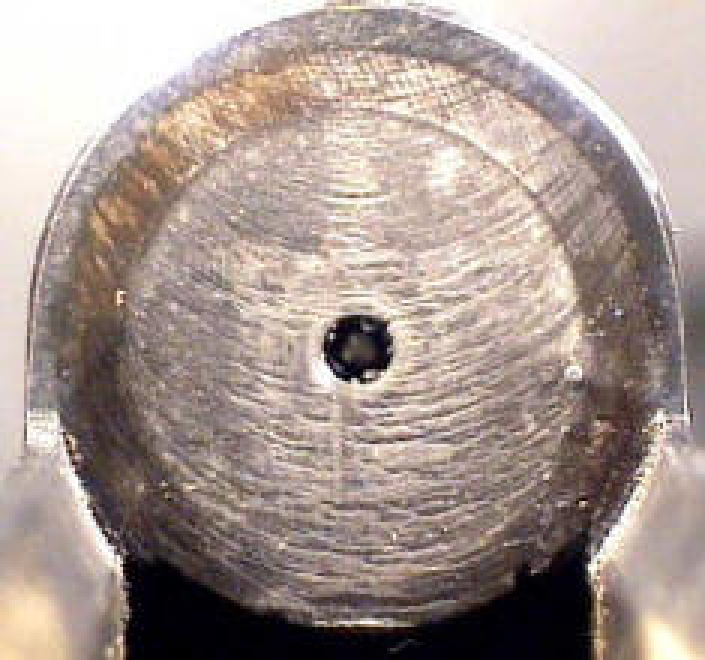
\includegraphics[width=.49\linewidth,height=2.5in]{../images/breechFace} }\subfloat[\label{figure:impressionsBF} Breech face impressions on a cartridge case primer\label{fig:impressionBF2}]{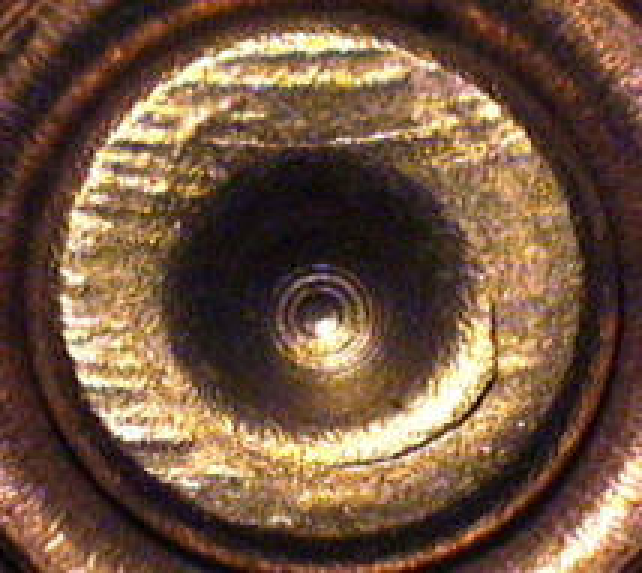
\includegraphics[width=.49\linewidth,height=2.5in]{../images/breechFaceImpression} }

}

\caption[Breech face of a barrel and breech face impression on a cartridge case \citep{doyle}]{Breech face of a barrel and breech face impression on a cartridge case \citep{doyle}}\label{fig:impressionBF}
\end{figure}
\end{Schunk}

These breech face impressions are considered to be analogous to a
firearm's ``fingerprint'' left on a cartridge case. Matching an expended
cartridge case of unknown source to one of known source based on breech
face impressions has been performed for over 100 years by forensic
practitioners \citep{firearm_id_thompson}. The development of
computational and statistical methods to perform such identification has
recently grown in interest \citep{council_strengthening_2009}.

One such method is the Congruent Matching Cells (CMC) method developed
at NIST that involves partitioning a cartridge case image or scan into a
grid of ``correlation cells" to isolate areas containing identifying
breech face impression markings \citep{song_proposed_2013}. Since its
invention in 2012, researchers at NIST have developed a number of
extensions and improvements of the CMC method. However, to date there
does not exist an openly available implementation of any of these
techniques. Rather, many methods described in the CMC literature include
a qualitative description of a proposed technique followed by results
from the authors' implementation. The description of these methods do
not delve into the intricacies of the implementation, which makes it
especially difficult to validate or assess. Additionally, some
procedures related to pre-processing the cartridge case data are
seemingly done by-hand at NIST rather than with an automated method.
This compounds the difficulty to accurately reproduce results. The
\pkg{cmcR} package provides an open-source, fully-automatic
implementation of the CMC method as originally described as well an
extension known as the ``High CMC'' method proposed by
\citet{tong_improved_2015}.

\hypertarget{data}{%
\subsection{Cartridge case data}\label{data}}

Cartridge case data commonly come in two forms: 2D grayscale images and
3D topographical scans. It is common in the CMC literature to use the 3D
topographical scans to demonstrate the efficacy of a proposed method
{[}\citep{tong_improved_2015}, \citep{chen_convergence_2017}{]}. A
variety of scans are openly available for download through the NIST
Ballistics Toolmark Research Database \citep{nbtrd}. The \pkg{cmcR}
package was designed specifically for use with the 3D topographies.

The 3D topographies are commonly stored in an .x3p (XML 3D Surface
Profile) file format that includes metainformation such as who took the
scan and the parameters under which the scan was taken (e.g., the
lateral resolution in microns). The \pkg{x3ptools} package in R provides
an interface to manipulate and visualize these .x3p files
\citep{x3ptools}. The physical surface is represented using a
\dfn{surface matrix}: a matrix of spatially-ordered elements or
``pixels" whose values correspond to the height of the cartridge case
surface at a particular location. Figure \ref{fig:cartridgeCasePair}
shows the surface matrices of a known match (KM) pair of cartridge
cases, meaning there were fired from the same firearm. Note that white
regions in the images below represent unobserved or missing values. When
read into R using the \pkg{x3ptools} package, these elements are encoded
as \code{NA}. The size of a surface matrix depends on the lateral
resolution with which the scans were taken. For example, a popular set
of scans in the CMC literature were taken by
\citet{fadul_empirical_nodate}; two of which are shown is the scan shown
in Figure \ref{fig:cartridgeCasePair}. These scans were taken with a
lateral resolution of 6.25 microns per pixel. The actual surface
matrices from this study vary around \(1200 \times 1200\) pixels in
size.

\begin{Schunk}
\begin{figure}[htbp]

{\centering \subfloat[\label{fig:rawBFs1}]{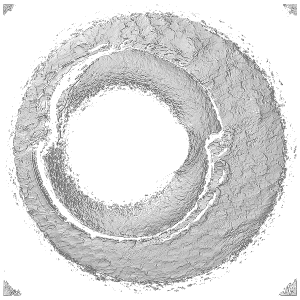
\includegraphics[width=.49\linewidth,height=.49\linewidth]{../images/fadul1-1} }\subfloat[\label{fig:rawBFs2}]{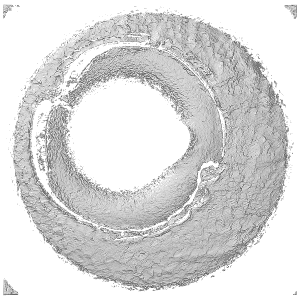
\includegraphics[width=.49\linewidth,height=.49\linewidth]{../images/fadul1-2} }

}

\caption{\label{fig:cartridgeCasePair} Two known match cartridge case scans from \citet{fadul_empirical_nodate}}\label{fig:rawBFs}
\end{figure}
\end{Schunk}

Only certain regions of a cartridge case contain identifying breech face
impression markings. \citet{song_proposed_2013} refers to these as
``valid correlation regions" that are to be used to determine whether
two cartridge cases match. The cell-based comparison procedure described
in section \protect\hyperlink{comparisonProcedure}{3.1} is designed to
emphasize such regions. However, prior to applying this procedure
cartridge scans must undergo some pre-processing to remove sections of
the cartridge case surface that do not come into contact with the breech
face of the barrel. These include a circular plateaued region in the
center of the scan that is pushed aside by the firing pin during the
firing process and clusters of observed values in the corners of the
scan that are artifacts of the staging area in which the scan was
captured. The task in pre-processing is to automatically remove these
unwanted regions from the scan to accentuate unique markings left by the
breech face. This is discussed in greater detail in section (LINK).

\hypertarget{cell-based-surface-matrix-comparisons}{%
\subsection{Cell-based surface matrix
comparisons}\label{cell-based-surface-matrix-comparisons}}

\hypertarget{comparisonProcedure}{%
\subsubsection{Cell-based comparison
procedure}\label{comparisonProcedure}}

The Congruent Matching Cells method was developed at the National
Institute of Standards and Technology to quantify the similarity between
two spent cartridge cases based on their breech face impressions. The
CMC method involves dividing a breech face impression scan into a grid
of cells and comparing each cell in one scan to a corresponding region
in the other scan. This method is motivated by the fact that breech face
markings are not uniformly impressed upon the cartridge case during the
firing process. As such, only certain sections of the cartridge case
have identifiable markings that make it possible to match to a firearm.
Calculating a similarity score between the entirety of two cartridge
case surfaces might not highlight these identifying regions. Instead,
the number of highly similar cell pairs between the two scans can be
used as a more granular similarity metric.

\begin{Schunk}
\begin{figure}[htbp]

{\centering 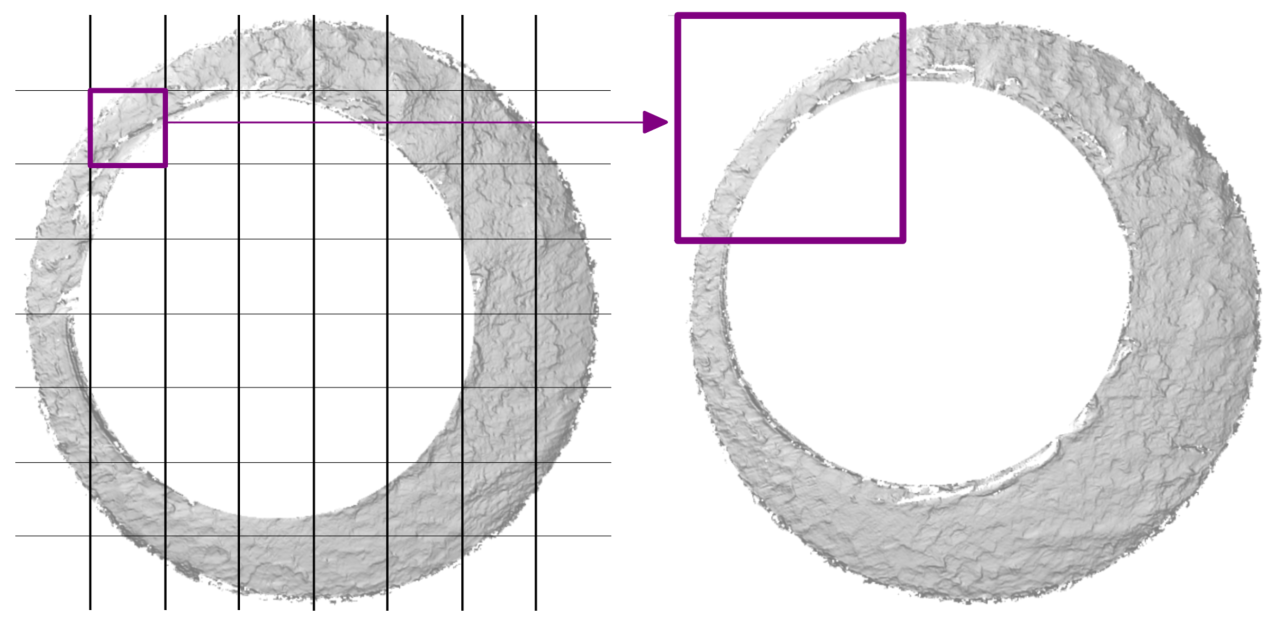
\includegraphics[width=\textwidth]{../images/cmc_illustration} 

}

\caption{\label{fig:cmc_illustration} Illustration of comparing a "cell" in one cartridge case scan to a region in another}\label{fig:unnamed-chunk-1}
\end{figure}
\end{Schunk}

Figure \ref{fig:cmc_illustration} illustrates the cell-based comparison
procedure between two cartridge case scans. The scan on the left is
divided into a grid of \(8 \times 8\) cells. Each cell is paired with an
associated larger region in the other scan. The absolute location of
each cell and region in their respective surface matrices remain
constant. However, the scan on the right is rotated to determine the
rotation at which the two scans are the most ``similar,'' which is
quantified using the \dfn{cross-correlation function} (CCF). For two
real-valued, \(M \times N\) matrices \(A\) and \(B\), the
cross-correlation function, denoted \((A \star B)\) can be defined as \[
(A \star B)[m,n] = \sum_{i=0}^M \sum_{j=0}^N A[i,j] B[(i + m)_{\text{mod}\ M}, (j + n)_{\text{mod}\ N}].
\] Note that this finite, discretized CCF is a matrix of elements
representing the similarity between matrices \(A\) and \(B\) for various
translations of matrix \(B\). The index at which the CCF attains a
maximum represents the translations needed to align \(B\) with \(A\). In
practice, calculating the CCF from the definition is often
computationally intractable. The \emph{Cross-Correlation Theorem}
provides a feasible alternative to calculating the CCF. For two matrices
\(A\) and \(B\), the Cross-Correlation Theorem says that \[
(A \star B )[m,n]= \mathcal{F}^{-1}\left(\overline{\mathcal{F}(A)} \cdot \mathcal{F}(B)\right)[m,n]
\] where \(\mathcal{F}\) and \(\mathcal{F}^{-1}\) denote the discrete
Fourier and inverse discrete Fourier transforms, respectively
\citep{fft_brigham}. Note that the multiplication on the right-hand side
is pointwise (Hadamard) multiplication. This result allows us to trade
the moving sum computations from the definition of the CCF for two
forward Fourier transformation, a pointwise product, and an inverse
Fourier transformation. The Fast Fourier Transform (FFT) algorithm is
used to reduce the computational load considerably. However, a practical
consideration for applying this method with cartridge case data is the
large number of non-random missing values in a surface matrix. Recall
that missing values are represented in Figures
\ref{fig:cartridgeCasePair} and \ref{fig:cmc_illustration} as white
pixels. The discrete Fourier transform is not defined for matrices
containing missing values, so these need to be replaced. The convention
adopted in the \pkg{cmcR} package is to replace missing values with 0
after standardizing a matrix by subtracting away its average height
value and dividing by its standard deviation. Such standardization is
commonly performed by authors at NIST {[}for example,
\citep{ott_applying_2017}{]}. While replacing missing values is
essential for using the FFT-based method of calculating the CCF, doing
so causes the CCF values to be ``deflated" relative to the
pairwise-complete cross-correlation in which only pairs of pixels in
which neither element is missing are considered. However, the
translation estimates obtained from this method are often good estimates
for true translation values by which the two matrices align.

Figure \ref{fig:ccfMap_example} provides an example of the output from
the FFT-based CCF calculation method. In the top-left we see a
\(72 \times 72\) pixel cell from one surface matrix. In the top-right we
see this cell's associated region in the other surface matrix of
dimension \(216 \times 216\) (triple the cell's side lengths). The
bottom-left shows the CCF ``map'' calculated using this FFT-based
method. Although the CCF need not be bounded between \(-1\) and \(1\)
based on the definition, it is common to normalize the CCF for
interpetability purposes and is done so in the \pkg{cmcR} package. A
summary of the alignment parameters at which the CCF\(_{\max}\) occurs
is shown in the bottom-right. We can see that the two matrices are
best-aligned when the cell is shifted ``east'' 20 pixels and ``north" 9
pixels starting from the center of the region. The \(\theta = -18\)
indicates that the overall cartridge case scan from which the region
(shown in the top-right) was extracted was rotated by \(-18\) degrees
for this comparion. The orange square in the top-right plot shows where
the cell would be located if the translation were performed.

\begin{Schunk}
\begin{figure}[htbp]

{\centering 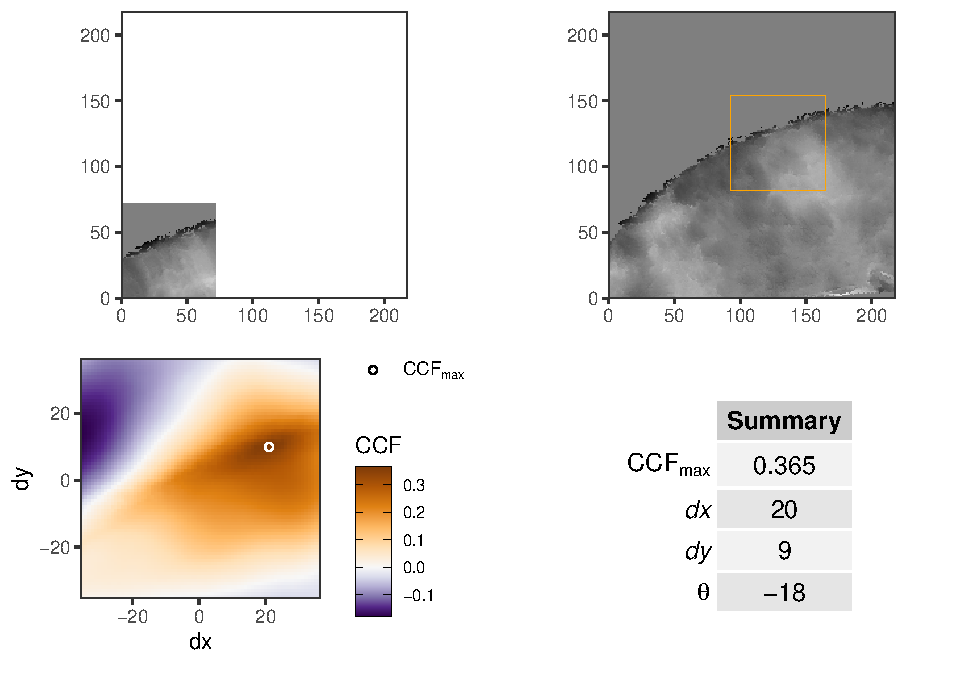
\includegraphics[width=\linewidth]{cmcR_files/figure-latex/unnamed-chunk-2-1} 

}

\caption{\label{fig:ccfMap_example} Example of a cross-correlation function "map" for a particular cell/region comparison}\label{fig:unnamed-chunk-2}
\end{figure}
\end{Schunk}

Using the estimated translation values at which the CCF\(_{\max}\)
occurs, we can calculate the pairwise-complete cross-correlation between
the cell and a cell-sized matrix extracted from the larger region where
missing values are not replaced. Think of this as punching-out the
matrix enclosed in the orange square shown in the top-right plot of
Figure \ref{fig:ccfMap_example}. This will be used as the final
CCF\(_{\max}\) estimate. This cell-based comparison procedure is
performed for each cell/region pair for various rotation values.

\hypertarget{the-congruent-matching-cells-method}{%
\subsection{The Congruent Matching Cells
method}\label{the-congruent-matching-cells-method}}

A particular cell/region pair is deemed ``highly similar'' if it passes
a collection of user-defined similarity criteria. The criteria are based
on the fact that a pair of matching cartridge case scans are not
necessarily aligned properly in their raw format. In particular, one
cartridge case scan needs to be rotated and translated to align
correctly the other. These unknown alignment parameters can be estimated
for each cell/region pair using the cell-based comparison procedure
discussed in section \protect\hyperlink{comparisonProcedure}{3.1}. For a
truly matching pair of cartridge cases, we would expect these alignment
parameter estimates to agree with each other across cell/region pairs;
at least up to some threshold. Conversely, we would expect the estimates
to vary randomly for a truly \emph{non}-matching pair. As such, the CMC
method details how to determine whether a consensus exists among the
estimated alignment parameter values across the cell/region pairs.

Since the initial proposal of the CMC method, a number of improvements
and extensions have been discussed by various authors. The \pkg{cmcR}
package provides an implementation for the initally proposed method as
well one extension proposed by \citet{tong_improved_2015} later referred
to as the ``High CMC'' method.

{[}Will be re-writing the explanation of both of these methods{]}

\hypertarget{the-initially-proposed-method}{%
\subsubsection{The initially proposed
method}\label{the-initially-proposed-method}}

In their raw format, a pair of matching cartridge case scans are not
necessarily properly aligned. If the surface matrices of two scans were
stacked on top of one another such that their centers coincided, one
would likely need to be rotated and translated to achieve maximum
similarity with the other. Once this is accomplished, an accurate
similarity score can be calculated between the two scans. For two scans
\(A\) and \(B\), let
\(\pmb{\beta} = (dx, dy, \theta)' \in \mathbb{R} \times \mathbb{R} \times [0,2\pi)\)
denote the translations and rotation needed to properly align \(A\) to
\(B\) (so \(-\pmb{\beta}\) would align \(B\) to \(A\)). For the CMC
method, we divide \(A\) into \(n\) cells and pair each cell with a
region in \(B\). As illustrated in Figure \ref{fig:cmc_illustration},
the regions in \(B\) are defined based on the location of their
associated cell in \(A\), yet with larger side lengths.

Each cell will have an associated
\(\pmb{\beta}_i = (dx_i, dy_i, \theta_i)', i = 1,...,n\), by which it
will achieve maximum similarity to the corresponding region in \(B\). If
\(A\) and \(B\) are truly matching (were fired from the same firearm),
then we would expect \(\pmb{\beta}_i = \pmb{\beta}\) for each \(i\). Due
to the unknowable nature of \(\pmb{\beta}\), the best we can hope to
determine is if \(\pmb{\beta}_i = \pmb{\beta}_j, i \neq j\). That is,
one criterion specified to call a pair of cartridge case scans a match
is that their cells' alignment parameters must agree. For non-matches,
we would not expect the \(\{\pmb{\beta}_i\}_{i = 1,...,n}\) to agree in
this way but rather to differ randomly. Note that, as shown in Figure
\ref{fig:cmc_illustration}, some cells contain little to no observed
values; for example, the corner cells of the Image 1 scan. Such cells
are not considered when determining similarity, although some vaguity
exists in how one might define a threshold to classify a particular cell
as containing too few observed values. For example,
\citet{chen_convergence_2017} only consider cells containing 15\% or
more observed values.

Because the cartridge cases are represented digitally, it is impossible
to search over every possible value of \(\pmb{\beta}_i\). Instead, the
alignment criterion, \(\pmb{\beta}_i = \pmb{\beta}_j, i \neq j\), is
applied to estimates for the alignment parameters,
\(\{\hat{\pmb{\beta}}_i\}_{i = 1,...,n}\). The translation parameter
estimates are determined using the maximum of the cross-correlation
function (CCF). This is effectively a template-matching procedure,
borrowing terminology from image processing, using the CCF as a
similarity metric. The rotation parameter esimate is determined through
a grid search. The method provides some estimation leeway by specifying
a threshold, \(\pmb{T} = (T_{dx}, T_{dy}, T_\theta)'\), within which we
say that two \(\hat{\pmb{\beta}}_i\)s agree. The CCF is also used to
quantify similarity between two cells analogous to how correlation can
be used to measure the linear relationship between two random variables.
In fact, a normalized CCF bounded between -1 and 1 is commonly
considered for interpretability. An additional criterion to classify a
cell pair as matching is a minimum CCF threshold, \(T_{CCF}\). Note that
these thresholds differ between authors (SOURCES).

In summary, the rotation parameter \(\theta\) is estimated by comparing
scan \(A\) to scan \(B\) over a grid of rotations of scan \(B\). For
each rotation of \(B\), each cell in \(A\) is compared to its associated
region in \(B\) using the CCF. This comparison yields both a maximum
cross-correlation function value and an estimate of \((dx,dy)'\) for
that particular rotation value. The method as initially proposed keeps
track of the estimated alignment parameters by which each cell in scan
\(A\) achieves its maximum CCF with the associated region in scan \(B\).
That is, each cell gets a single ``vote'' for the
\(\hat{\pmb{\beta}}_i\) that provides the best alignment between it and
its associated region in scan \(B\). Cells that contain too few observed
values aren't given a vote. A ``consensus'' is determined by aggregating
in some way the \((dx,dy,\theta)'\) votes. For example, the median of
the \((dx,dy,\theta)'\) estimates may be taken as the consensus. The
votes of each cell are then compared to this consensus to determine if
they are within the \((T_{dx}, T_{dy}, T_\theta)'\) thresholds. Any cell
whose \(\hat{\pmb{\beta}}_i\) vote fall within these thresholds and
whose maximum CCF is above the specified \(T_{CCF}\) threshold is
classified as a ``congruent matching cell.''

\hypertarget{highCMCMethod}{%
\subsubsection{The High CMC method}\label{highCMCMethod}}

\citet{tong_improved_2015} discuss an improved version of the CMC method
that targets specific deficiencies in the initially proposed method.
Namely, the fact that each image \(A\) cell gets only one vote for the
\((dx,dy,\theta)'\) alignment parameters by which it achieves maximum
similarity with its associated region in image \(B\). A cell pair may be
wrongfully excluded from the ``congruent matching cell'' classification
because, for example, the rotation for which it votes falls too far from
the consensual rotation value. In reality, the cell pair may be highly
similar at the consensual rotation value, yet is never given the chance
to demonstrate this. The improved version of the method attempts to
effectively give such cell pairs a second chance by considering their
behavior at the consensual rotation value; although it introduces an
additional criterion to guard against the possibility of a non-matching
cell pair being highly similar by chance at the consensual rotation
value.

This additional criterion is based on an observation that appears to be
true based on empirical evidence: if a pair of cartridge case scans
\(A\) and \(B\) are truly matching after rotating \(B\) by \(\theta\),
then they should still be highly similar after rotating \(B\) by
\(\theta + \epsilon\) for some small \(\epsilon\). In terms of the CMC
method, this means that the number of congruent matching cell pairs
should reach a mode at the true \(\theta\) value. In practice, because
only a grid of \(\theta\) values are considered, a mode is detected
based on how close the \(\theta\) values yielding a high number of CMCs
are to each other. Tong et al.~classifies a ``high" number of CMCs as
CMC\(_{\max} - \tau\) where CMC\(_{\max}\) is the maximum number of CMCs
detected across all \(\theta\) values and \(\tau\) is an empirical
constant (\(\tau = 1\) in \citet{tong_improved_2015}).

Another improvement to the original method proposed by Tong et al.~is to
consider both a comparison of scan \(A\) to rotated versions of scan
\(B\) as well as \(B\) to \(A\). The motivation for this being that true
matches should be highly similar in either direction while non-matches
should have conflicting or random results. Figure
\ref{fig:kmCMCPerTheta} shows the ``forward'' and ``backward'' CMC count
distribution for a known match pair across a grid of rotation values,
\(\theta \in \{-30,-27,...,27,30\}\). We can see that both distributions
achieve a mode at opposite \(\theta\) values, which is expected and
desired for a known match pair. Additionally, a horizontal line has been
drawn at CMC\(_{\text{high}} =\) CMC\(_{\max} - 1\) for the respective
distributions. We can see that in either case, any \(\theta\) value that
achieves this CMC\(_{\text{high}}\) value is close to the mode. In
contrast, Figure \ref{fig:knmCMCPerTheta} shows the CMC count
distribution for a known non-match pair that is relatively flat. In
particular, we see that there are \(\theta\) values achieving
CMC\(_{\text{high}}\) that are far away from the mode.

\begin{Schunk}
\begin{figure}[htbp]

{\centering 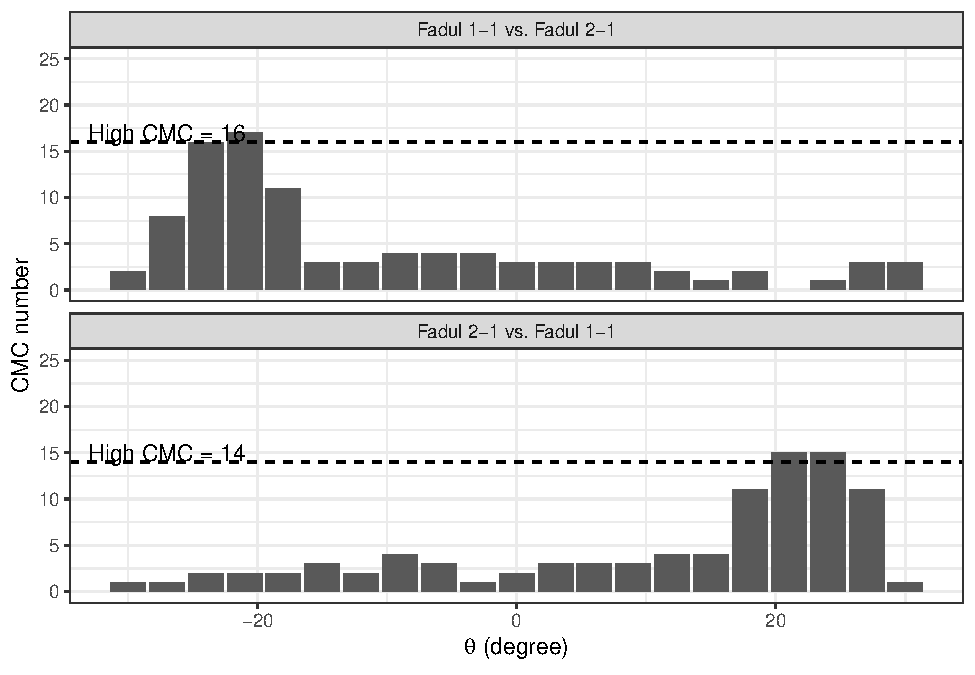
\includegraphics[width=.7\textwidth]{cmcR_files/figure-latex/unnamed-chunk-3-1} 

}

\caption{\label{fig:kmCMCPerTheta} CMC count per rotation ($\theta$) value for forward (x3p1 vs. x3p2) and backward (x3p2 vs. x3p1) comparison of a known match cartridge case pair}\label{fig:unnamed-chunk-3}
\end{figure}
\end{Schunk}

\begin{Schunk}
\begin{figure}[htbp]

{\centering 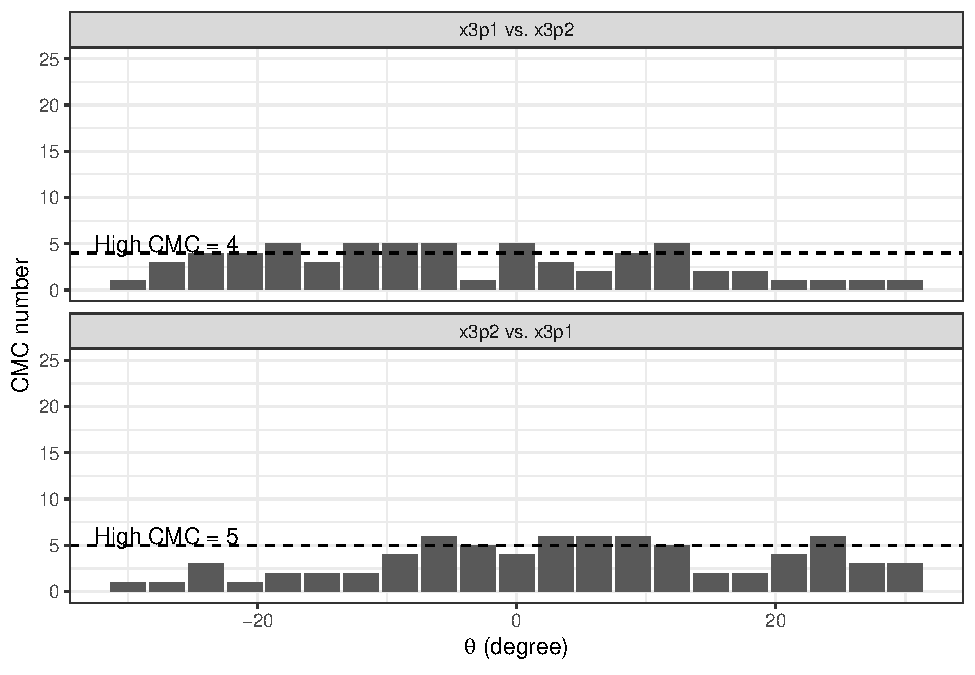
\includegraphics[width=.7\textwidth]{cmcR_files/figure-latex/unnamed-chunk-4-1} 

}

\caption{\label{fig:knmCMCPerTheta} CMC count per rotation ($\theta$) value for forward (x3p1 vs. x3p2) and backward (x3p2 vs. x3p1) comparison of a known non-match cartridge case pair}\label{fig:unnamed-chunk-4}
\end{figure}
\end{Schunk}

These additional ``high CMC count" criteria provide more enhanced
discriminatory ability between known matching and known non-matching
scans. If this criterion is satisfied by a particular pair of scans and
a \(\theta\) mode is identified, then the method considers CCF values
for each cell pair at and around this mode. Again, this is in contrast
to the initially proposed method that only considers the CCF\(_{\max}\)
value and resulting \((dx,dy,\theta)\) votes for each cell pair.

\hypertarget{the-package}{%
\subsection{\texorpdfstring{The \pkg{cmcR}
package}{The  package}}\label{the-package}}

This section will highlight the \pkg{cmcR} package's functionality by
walking through a possible use case. Many of the functions in this
package provide the user with a variety of processing options with which
they can experiment. This is due to the fact that processing techniques
differ considerably among authors or are not discussed in great detail.

\hypertarget{pre-processing-procedures}{%
\subsubsection{Pre-processing
procedures}\label{pre-processing-procedures}}

Studies in which cartridge cases are matched by forensic examiners often
involve giving examiners a set of known matches and asking them to
classify additional matches from a collection of unknown source scans.
For brevity, we will consider a comparison between two cartridge cases.
This particular pair of scans, as well as many other cartridge case
scans, are openly available from the NIST Ballistics and Toolmarks
Research Database. Figure \ref{fig:processedScans} shows the pair of
scans after performing the necessary pre-processing procedures. Note
that the color scheme has been scaled by quantiles to visually highlight
regions of the cartridge case scan containing strong breech face
impression ``signal.''

\begin{Schunk}
\begin{figure}[htbp]

{\centering 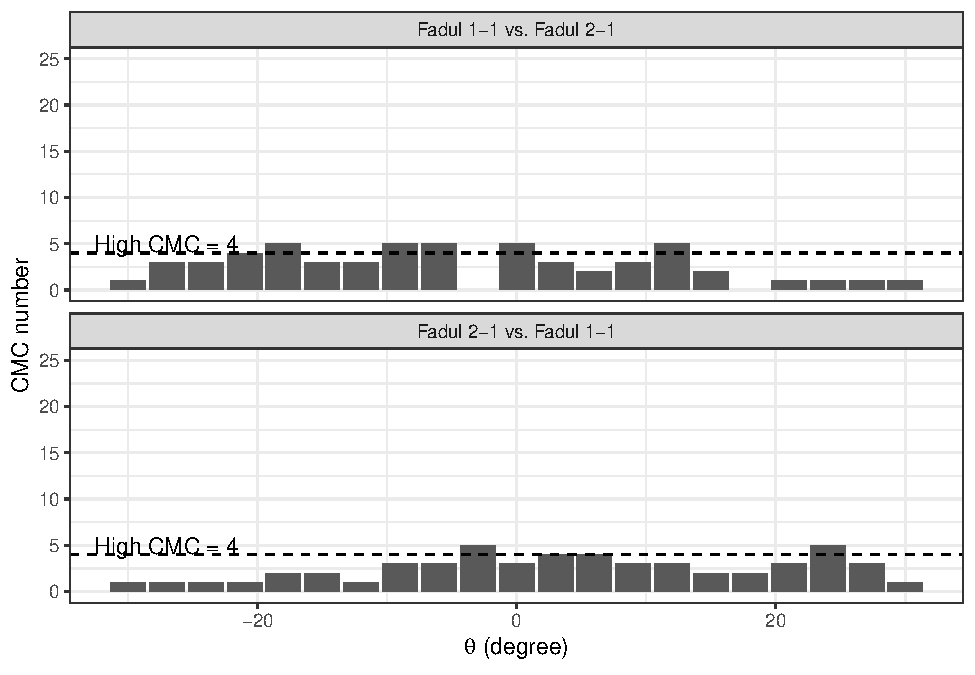
\includegraphics[width=1.2\textwidth,trim={0 2.5cm 0 2cm}]{cmcR_files/figure-latex/unnamed-chunk-5-1} 

}

\caption{\label{fig:processedScans} A known match pair of processed cartridge case scans}\label{fig:unnamed-chunk-5}
\end{figure}
\end{Schunk}

The family of functions in the \pkg{cmcR} package beginning with
\code{preProcess\_} can be used to perform the necessary pre-processing
steps for a pair of cartridge case scans to be comparable using the
cell-based comparison procedure outlined in section
\protect\hyperlink{comparisonProcedure}{3.1}. The implementation of many
of these pre-processing procedures is inspired largely by
\citet{tai_fully_2018} who detail a fully-automatic procedure for
processing cartridge case 2D images as opposed to 3D scans. The
functions available include:

\begin{enumerate}
\item \code{preProcess\_ransac}: estimates the height value of the breech face impressions in a scan using the Random Sample Consensus (RANSAC) robust, iterative plane-fitting algorithm \citep{ransac}.

\item \code{preProcess\_levelBF}: extracts the observations containing breech face impressions from the scan using the estimated height value obtained from \code{preProcess\_levelBF}.

\item \code{preProcess\_cropWS}: removes rows/columns containing mostly if not all \code{NA} values from the surface matrix on the exterior of breech face impressions.

\item \code{preProcess\_removeFPCircle}: detects and removes observations within the firing pin impression circle using the Hough Transform circle detection algorithm \citep{hough}.

\item \code{preProcess\_gaussFilter}: applies a low-pass, high-pass, or band-pass Gaussian filter to the breech face impressions to reduce the effects of high frequency noise, low frequency global structure, or both, respectively.
\end{enumerate}

See the \pkg{cmcR} package documentation for more information about
these functions.

For computational purposes it is common the CMC literature to
down-sample a surface matrix prior to performing the cell-based
comparison procedure. The \code{sample\_x3p} function from the
\pkg{x3ptools} package can be used used to sample every \(m\)th
row/column of a surface matrix. Together with the \code{preProcess\_}
family of functions, the code to produce the first surface matrix shown
in Figure \ref{fig:processedScans} is given by the following example.

\begin{Schunk}
\begin{Sinput}
library(cmcR)
library(x3ptools)
library(magrittr)

nrbtd_url <- "https://tsapps.nist.gov/NRBTD/Studies/CartridgeMeasurement/"

fadul1.1_id <- "DownloadMeasurement/2d9cc51f-6f66-40a0-973a-a9292dbee36d"
fadul1.2_id <- "DownloadMeasurement/cb296c98-39f5-46eb-abff-320a2f5568e8"

fadul1.1 <- read_x3p(file = paste0(nrbtd_url,fadul1.1_id)) %>%
  sample_x3p(m = 2)

fadul1.1$surface.matrix <- fadul1.1$surface.matrix %>%
  #first RANSAC estimation yields rough height estimate
  preProcess_ransac(inlierTreshold = 1e-6, #1 micrometer
                    iters = 150) %>%
  preProcess_levelBF() %>%
  #second, more precise RANSAC estimation
  preProcess_ransac(inlierTreshold = 1e-7,
                    iters = 300) %>%
  preProcess_levelBF() %>%
  preProcess_cropWS(croppingThresh = 1) %>%
  preProcess_removeFPCircle() %>%
  #Gaussian band-pass filter
  preProcess_gaussFilter(res = fadul1.1$header.info$incrementY,
                         wavelength = c(16,250),
                         filtertype = "bp")
\end{Sinput}
\end{Schunk}

\subsection{Implementation of cell-based comparison procedure}

The cell-based comparison procedure outlined in section
\protect\hyperlink{comparisonProcedure}{3.1} is implemented in the
\code{cellCCF\_bothDirections} function. In particular, the procedure is
performed twice so that both cartridge case scans take on the role of
the scan that is partitioned into a grid of cells. This is necessary to
apply the High CMC logic discussed in section
\protect\hyperlink{highCMCMethod}{3.2.2}. Continuing with the current
use case example, the code to perform this procedure on \code{fadul1.1}
and \code{fadul1.2} is given by the following example.

\begin{Schunk}
\begin{Sinput}
kmComparison <- cellCCF(x3p1 = fadul1.1,
                        x3p2 = fadul1.2,
                        thetas = seq(-30,30,by = 3),
                        cellNumHoriz = 8,
                        cellNumVert = cellNumHoriz)
kmComparison$comparison_1to2$ccfResults$`3` %>%
  head()
\end{Sinput}
\end{Schunk}

\begin{Schunk}
\begin{table}[!h]

\caption{\label{tab:unnamed-chunk-8}\label{tab:cellCCF} Example of output from \code{cellCCF} function}
\centering
\begin{tabular}[t]{r|l|r|r|r|r|r}
\hline
cellNum & cellID & ccf & fft.ccf & dx & dy & theta\\
\hline
2 & y = 1 - 73, x = 74 - 145 & 0.7762319 & 0.2108462 & 34 & -30 & 3\\
\hline
3 & y = 1 - 73, x = 146 - 217 & 0.1006877 & 0.1145874 & 29 & 22 & 3\\
\hline
4 & y = 1 - 73, x = 218 - 289 & 0.1863672 & 0.1030728 & -32 & -16 & 3\\
\hline
5 & y = 1 - 73, x = 290 - 362 & 0.8004083 & 0.3658809 & 5 & 4 & 3\\
\hline
6 & y = 1 - 73, x = 363 - 434 & 0.7036884 & 0.2353348 & 22 & 10 & 3\\
\hline
7 & y = 1 - 73, x = 435 - 506 & 0.7965972 & 0.1407746 & -25 & -18 & 3\\
\hline
\end{tabular}
\end{table}

\end{Schunk}

\hypertarget{congruent-matching-cells-logic}{%
\subsection{Congruent Matching Cells
logic}\label{congruent-matching-cells-logic}}

{[}Pretty much full re-write of this section{]}

With the CCF results calculated across a range of rotation values, we
can extract the features used in the Congruent Matching Cells method.

The \code{cmcR::topResultsPerCell} function extracts from the list
returned by \code{cellCCF} information about the \((\theta,dx,dy)'\)
values at which each cell pair achieves its maximum CCF. The resulting
data frame is required for determining the number of CMCs under the
initially proposed method. Recall that the initially propsed method
filters this data frame down by determining which cell pairs have
associated \((\theta,dx,dy)'\) values close to the consensus
\((\theta,dx,dy)'\). Passing this data frame to the
\code{cmcR::cmcFilter} function implements this filtering process. The
\code{cmcFilter} function provides options to specify the function used
to form a consensus among \((\theta,dx,dy)'\) values and define
thresholds for calling a particular cell pair's \((\theta,dx,dy)'\)
values ``close" to the consensus. Optionally, separate consensus
functions can be defined for the \(\theta\) and \((dx,dy)'\) values.
This is motivated by the fact that, especially for a course grid, the
\(\theta\) values can be considered categorical while the \((dx,dy)'\),
although only ever observed as integers, should be treated as
continuous. The code below illustrates how CMCs under the initially
proposed method can be calculated. The \code{cmcR::getMode} function
calculates the mode \(\theta\) value among those in the
\code{topResultsPerCell} data frame.

\begin{Schunk}
\begin{Sinput}
comparison1$ccfResults %>%
  topResultsPerCell() %>%
  cmcFilter(consensus_function = median,
            ccf_thresh = .55,
            dx_thresh = 35,
            dy_thresh = 35,
            theta_thresh = 3,
            consensus_function_theta = cmcR::getMode)
\end{Sinput}
\end{Schunk}

Table \ref{tab:initialCMC} shows the CMCs determined by the
\code{cmcFilter} function for the two comparisons made in the current
use case. We can see that the comparison between Unknown Source and
Known Source 1 yields more CMCs than the comparison with Known Source 2.
In fact, Song et al.~(2013) recommend a minimum of 6 CMCs before calling
a cartridge case pair a match. For this fabricated use case, Unknown
Source indeed matches to Known Source 1 while Known Source 2 is a known
non-match.

\begin{Schunk}
\begin{Sinput}
cmcPlots <- cmcR::cmcPlot(fadul1.1$x3p,
              fadul1.2$x3p,
              cellCCF_bothDirections_output = kmComparison,
              cmcFilter_improved_output = kmCMC)

cmcPlots$initialCMC
\end{Sinput}
\begin{Soutput}
#> [[1]]
\end{Soutput}

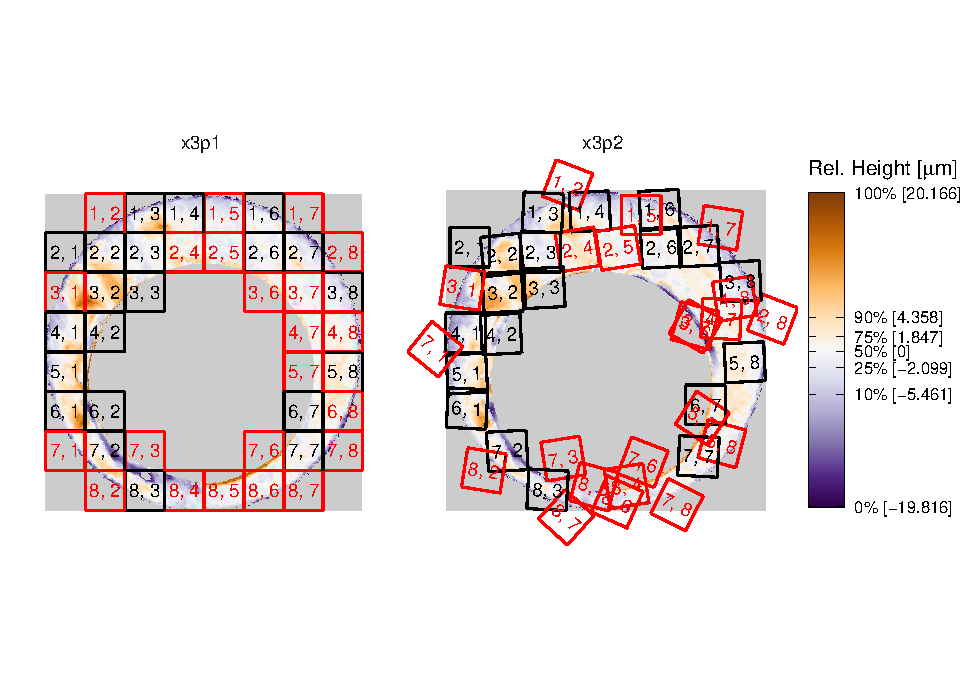
\includegraphics{cmcR_files/figure-latex/unnamed-chunk-10-1} \begin{Soutput}
#> 
#> [[2]]
\end{Soutput}

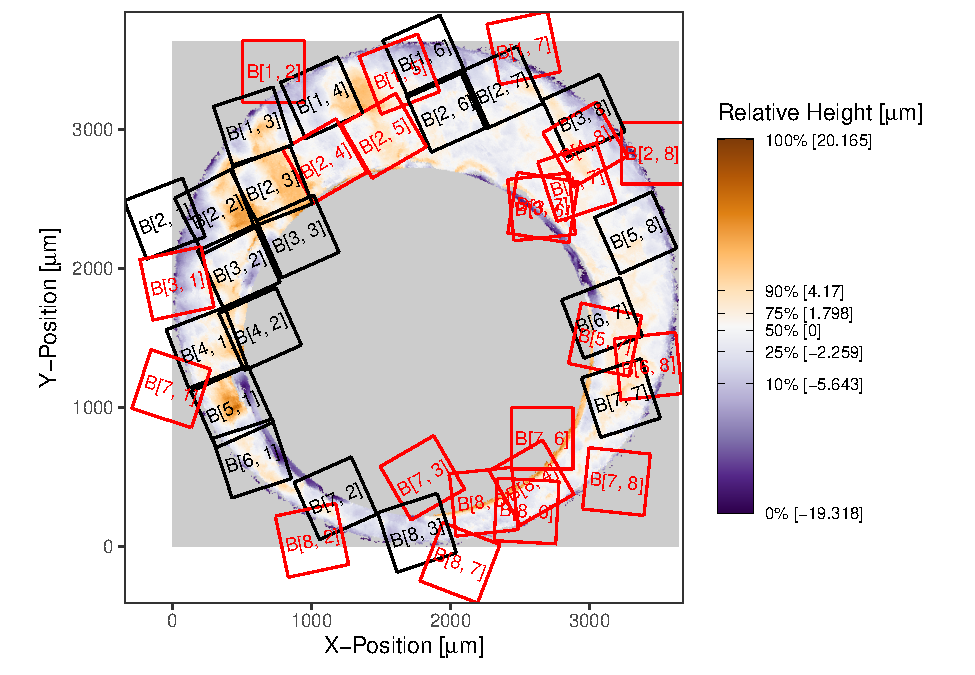
\includegraphics{cmcR_files/figure-latex/unnamed-chunk-10-2} 
\end{Schunk}

While useful for an initial estimate of the CMC count between two
cartridge case scans, the improved method as desribed in section (LINK)
has been shown to be more effective at classifiying matches from
non-matches. The \code{cmcR::cellCCF\_bothDirections} is just a wrapper
for calling \code{cellCCF} twice where the two x3p objects change roles
for the second call. The value returned by
\code{cellCCF\_bothDirections} is a list of two elements, the first
being the comparisons between \code{x3p1} to rotations of \code{x3p2}
and the second being the comparisons between \code{x3p2} to rotations of
\code{x3p1}. The output of \code{cellCCF\_bothDirections} can be handed
off to the \code{cmcR::cmcFilter\_improved} function to implement the
improved CMC method. The value returned by
\code{cmcR::cmcFilter\_improved} is a list of 3 elements. The first
element, \code{params}, contains the argument specifications under which
the function call was made. The second element, \code{initialCMCs},
contains two dataframes of the CMCs calculated under the initially
proposed method (equivalent to calling \code{cmcFilter} twice). The
third element, \code{finalCMCs}, contains a data frame with the CMCs
calculated under the improved method. If no additional CMCs are
determined using the improved method, then a cartridge case pair is
assigned the number of CMCs calculated under the initially proposed
method. Such is the case for the comparison between Unknown Source and
Known Source 2. Table \ref{tab:finalCMC} shows this table for the
current use case between Unknown Source and Known Source 1.

\begin{Schunk}
\begin{Sinput}
comparison2 <- cmcR::cellCCF_bothDirections(x3p1 = processedBF1$x3p,
                                            x3p2 = processedBF2$x3p,
                                            thetas = seq(-30,30,by = 3),
                                            cellNumHoriz = 8,
                                            cellNumVert = 8,
                                            centerCell = "wholeMatrix")

cmcR::cmcFilter_improved(cellCCF_bothDirections_output = comparison2,
                         consensus_function = median,
                         ccf_thresh = .5,
                         dx_thresh = 35,
                         dy_thresh = 35,
                         theta_thresh = 3,
                         consensus_function_theta = cmcR::getMode)
\end{Sinput}
\end{Schunk}

\begin{Schunk}
\begin{Sinput}
cmcPlots$finalCMC
\end{Sinput}
\begin{Soutput}
#> [[1]]
\end{Soutput}

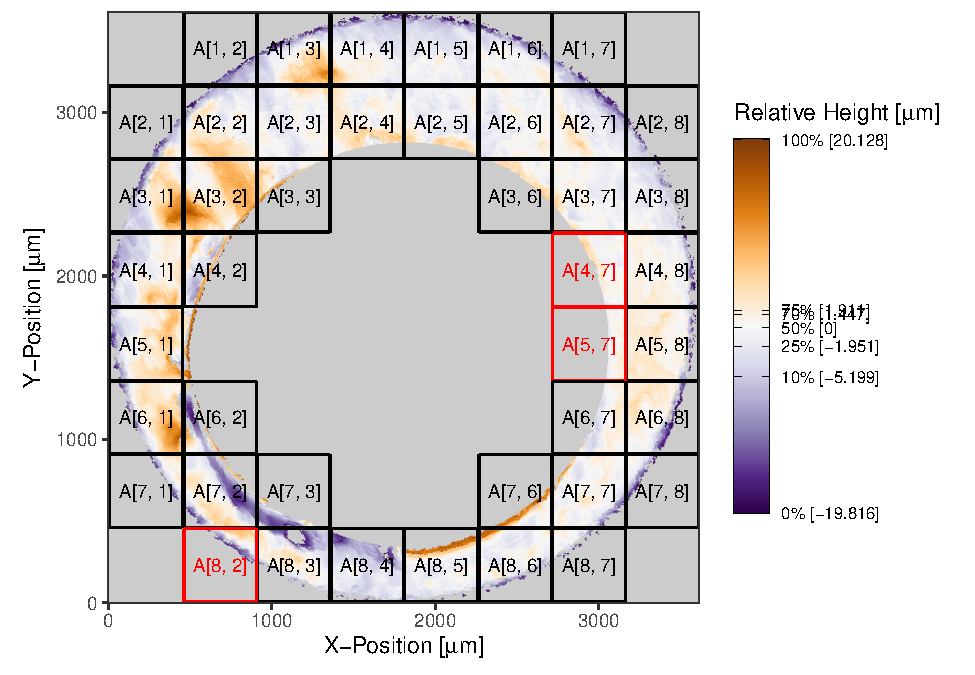
\includegraphics{cmcR_files/figure-latex/unnamed-chunk-12-1} \begin{Soutput}
#> 
#> [[2]]
\end{Soutput}

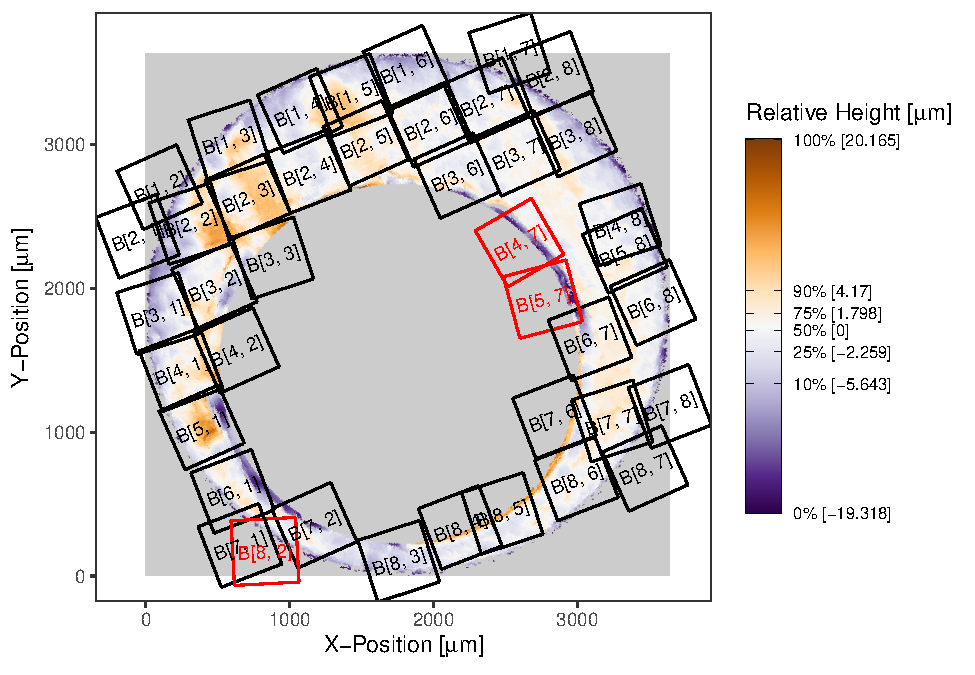
\includegraphics{cmcR_files/figure-latex/unnamed-chunk-12-2} 
\end{Schunk}

\bibliography{RJreferences}


\address{%
Joseph Zemmels\\
Iowa State University Department of Statistics\\
2438 Osborn Dr\\ Ames, IA 50011\\
}
\href{mailto:jzemmels@iastate.edu}{\nolinkurl{jzemmels@iastate.edu}}

\address{%
Heike Hofmann\\
Iowa State University Department of Statistics\\
2438 Osborn Dr\\ Ames, IA 50011\\
}
\href{mailto:hofmann@iastate.edu}{\nolinkurl{hofmann@iastate.edu}}

\address{%
Susan VanderPlas\\
University of Nebraska - Lincoln Department of Statistics\\
340 Hardin Hall North Wing\\ Lincoln, NE 68583\\
}
\href{mailto:susan.vanderplas@iastate.edu}{\nolinkurl{susan.vanderplas@iastate.edu}}

